
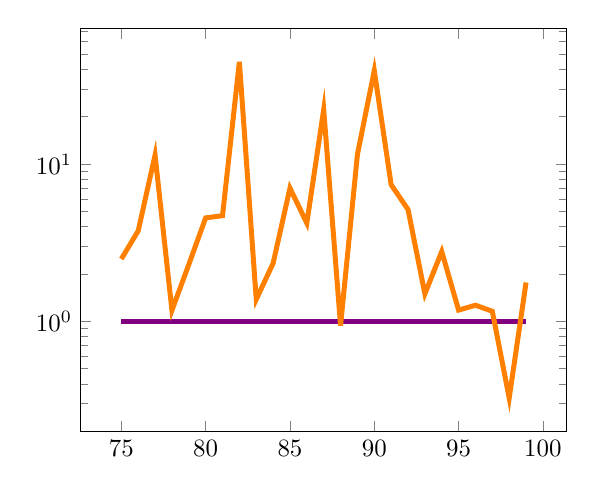
\begin{tikzpicture}[scale=0.9]
\begin{semilogyaxis}
\addplot[color=violet,line width=2pt] coordinates {(75,1.0)(76,1.0)(77,1.0)(78,1.0)(79,1.0)(80,1.0)(81,1.0)(82,1.0)(83,1.0)(84,1.0)(85,1.0)(86,1.0)(87,1.0)(88,1.0)(89,1.0)(90,1.0)(91,1.0)(92,1.0)(93,1.0)(94,1.0)(95,1.0)(96,1.0)(97,1.0)(98,1.0)(99,1.0)};
\addplot[color=orange,line width=2pt] coordinates {(75,2.4913141936439764)(76,3.75673198913989)(77,11.388308599677226)(78,1.174750958206233)(79,2.2948322760908426)(80,4.542720676366331)(81,4.693928178783805)(82,44.59273478710782)(83,1.3786318495858894)(84,2.33693666447023)(85,7.021100227746091)(86,4.206008657093421)(87,22.15963579854953)(88,0.940087684288178)(89,11.494410834697433)(90,39.19344027201383)(91,7.38208581754482)(92,5.1357924298046616)(93,1.4970641702314238)(94,2.7747660139048413)(95,1.178628738168884)(96,1.2660928166140892)(97,1.1581844253541862)(98,0.3255329718490719)(99,1.7658507629615088)};

\end{semilogyaxis}
\end{tikzpicture}
